% !TEX TS-program = pdflatex
% !TEX encoding = UTF-8 Unicode

\documentclass{beamer}
%\documentclass[handout]{beamer}

%\setbeamertemplate{background canvas}[vertical shading][bottom=white,top=structure.fg!25]
% or whatever

\usetheme[compress]{Amsterdam}
%\setbeamertemplate{headline}{}
%\setbeamertemplate{footline}{}
%\setbeamersize{text margin left=0.5cm}
  
\usepackage[english]{babel}
\usepackage{listings}
\usepackage{geometry}
\usepackage{hyperref}

\usepackage{color}
\usepackage[T1]{fontenc}
\usepackage[utf8]{inputenc}
\usepackage{lmodern}
\usepackage{etoolbox}

\usepackage{tikz}
\usetikzlibrary{shapes,arrows}

\usepackage{multicol}
\lstset{
basicstyle=\scriptsize\ttfamily,
columns=flexible,
breaklines=true,
numbers=left,
%stepsize=1,
numberstyle=\tiny,
backgroundcolor=\color[rgb]{0.85,0.90,1}
}


\begin{document}

\title[Big Data and Automated Content Analysis]{\textbf{A Practical Introduction to Machine Learning in Python} \\Day 5 - Friday \\ »Finding the best model and communicating results«}
\author[Damian Trilling, Anne Kroon]{Damian Trilling \\ Anne Kroon \\ ~ \\ \footnotesize{d.c.trilling@uva.nl, @damian0604 \\a.c.kroon@uva.nl, @annekroon} \\}
\date{March 13, 2020}
\institute[Gesis]{Gesis}


\tikzstyle{block} = [rectangle, draw, fill=blue!20, 
text width=5em, text centered, rounded corners, minimum height=4em]
\tikzstyle{line} = [draw]
\tikzstyle{pijltje} = [draw, -latex']
\tikzstyle{cloud} = [draw, ellipse,fill=red!20, node distance=3cm,
minimum height=2em, text width=4em, text centered,]



\setbeamercovered{transparent}

\begin{frame}{}
\titlepage
\end{frame}

\begin{frame}{Today}
\tableofcontents
\end{frame}




\section{Alternatives to train/test split}

\begin{frame}[plain]
\textbf{Alternatives to train/test split}

Train/validation/test split 
\end{frame}


\subsection{Train/validation/test split}

\begin{frame}{Train/validation/test split}
\begin{itemize}
\item When you compare a lot of different models (or (hyper-)parameters), you might want to evaluate (compare) them using a third dataset 
\item e.g., make 80/20 split (train/test); then split first part again 80/20 (train/validation)
\item only use the test data \emph{at the very end} to get a final estimate of how good your model is.
\end{itemize}
\pause
In short: Validation data to \emph{select} the best approach; test data to get the accuracy of the approach you chose.
\end{frame}

\subsection{Cross-validation}

\begin{frame}[plain]
\textbf{Alternatives to train/test split}

Cross-validation
\end{frame}

\begin{frame}[fragile]{Cross-validation}
\begin{lstlisting}
from sklearn.model_selection import cross_val_score
from sklearn.naive_bayes import MultinomialNB
nb = MultinomialNB()     # the classifier we trained last week
scores = cross_val_score(nb,  train_features, [r[1] for r in reviews], cv=10)
print(scores)
\end{lstlisting}

results in:

\begin{lstlisting}
[0.858  0.8612 0.8516 0.8528 0.8672 0.8664 0.8576 0.8652 0.8436 0.852 ]
\end{lstlisting}

In other words, we estimate the model 10 times on different trainig/validation data splits and get 10 different F1-scores (could be any other metric as well).

\end{frame}


\begin{frame}{Cross-validation}
\begin{block}{Why would we want to do that?}
\begin{itemize}
\item We could get some confidence interval around our scores
\item Does not ``waste'' too much validation data
\item \ldots and that's important for hyperparameter tuning
\end{itemize}

\end{block}

{\footnotesize See for more info
\url{https://scikit-learn.org/stable/modules/cross\_validation.html}}
\end{frame}





\section{Finding the optimal (hyper-)parameters}


\begin{frame}[plain]
\vspace{2cm}
\textbf{Finding the optimal (hyper-)parameters}

Grid-search
\vspace{2cm}

{\footnotesize 
\begin{description}
\item[\textcolor{red}{hyperparameter}] a parameter of a model that is not learned through training, but specified in advance
\end{description}
}
\end{frame}



\subsection{Hyperparameter optimization with grid search}

\begin{frame}{Hyperparameter optimization with grid search}
\begin{block}{General idea}
Rather than arbitrary trying some combinations of hyperparameters, let's systematically test and compare.
\end{block}

\pause

\begin{example}
\begin{itemize}[<+->]
\item To avoid overfitting, scikit-learn adds a \emph{regularization term} to the loss function that is minimized to fit the regression.
\item Think of this term as a penalty for too complex models
\item How much weight should our penalty carry? That's determined by a constant, $C$.
\item How to determine the best $C$? $\Rightarrow$ grid search 
\end{itemize}
\end{example}
\end{frame}


\begin{frame}[fragile]{Hyperparameter optimization with grid search}
Finding $C$ in a logistic regression using 5-fold cross-validation
\begin{lstlisting}
from sklearn.linear_model import LogisticRegressionCV
logregCV = LogisticRegressionCV(cv=5).fit(train_features, [r[1] for r in reviews])
\end{lstlisting}
\pause 

\begin{itemize}[<+->]
\item Here, we just need to use \texttt{LogisticRegressionCV} instead of \texttt{LogisticRegression}. 
\item But we can use it to test any combination of choices (example at \url{https://scikit-learn.org/stable/auto\_examples/model\_selection/grid\_search_text\_feature\_extraction.html})
\end{itemize}

\end{frame}

\begin{frame}{Grid-search takeaway}
\begin{itemize}[<+->]
\item When you want to systematically test what happens when you vary a hyperparameter, use grid-search to automatically do so and select the best value
\item sometimes already implemented (e.g., \texttt{LogisticRegressionCV} as direct replacement for \texttt{LogisticRegression})
\item But \texttt{GridSearchCV} is very flexible: can be used in combination with pipeline (wait a minute\ldots) for very different purposes
\end{itemize}


\end{frame}



\begin{frame}[plain]
\textbf{Finding the optimal (hyper-)parameters}

Tuning decision thresholds with ROC curves
\end{frame}

\subsection{Tuning decision thresholds with ROC curves}

\begin{frame}{From estimate to label}
\makebox[\linewidth]{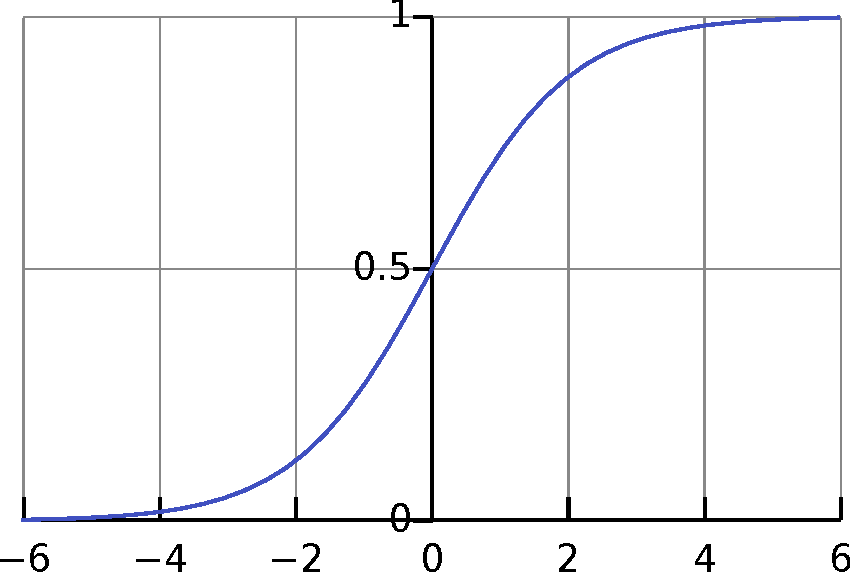
\includegraphics[width=.5\paperwidth,height=\paperheight,keepaspectratio]{../pictures/sigmoid}}
In logistic regression, we use the \textit{sigmoid function} to transform the estimates into probabilities.

To transform the probabilities into binary labels, we use a cutoff (default: 0.5).
\end{frame}

\begin{frame}{Why use 0.5 as cutoff?}
\begin{itemize}[<+->]
\item It makes most sense (intuitively, mathematically)
\item But remember our precision/recall tradeoff: maybe we want to be `stricter' or `less strict'
\item Maybe it is importance to us that our classifier is balanced and equally good in predicting both classes, even if overall accuracy suffers (slightly) 
\end{itemize}
\pause
Let's see what happens if we plot False Positives against True Positives (ROC-curve)
\end{frame}


\begin{frame}{ROC Curve}
\makebox[\linewidth]{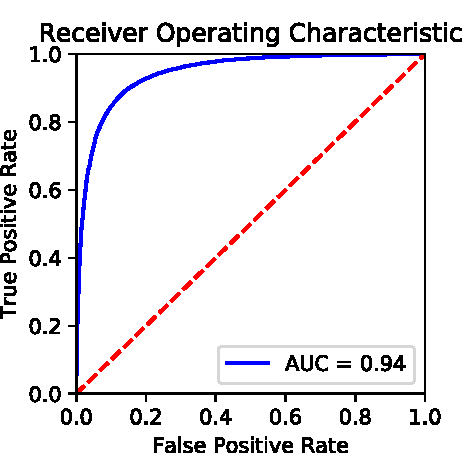
\includegraphics[width=.5\paperwidth,height=.5\paperheight,keepaspectratio]{../pictures/roccurve}}
\begin{itemize}
\item If we choose a threshold such that we get very little false positives, we also get too little true positives.
\item Optimum in the upper left corner
\end{itemize}

\end{frame}


\begin{frame}{So, how to we determine the exact value? }
See notebook

\url{https://github.com/damian0604/bdaca/blob/master/rm-course-2/week10/Determining\%20the\%20cutoff-point\%20in\%20logistic\%20regression.ipynb}
\end{frame}



\section{From feature set to final classification}

\subsection{Putting stuff together with pipelines}
\begin{frame}[plain]
\textbf{From feature set to final classification}

Putting stuff together with pipelines
\end{frame}

\begin{frame}{A pipeline}
\begin{itemize}
\item Machine learning involves multiple steps (e.g., preprocessing $\rightarrow$ vectorizer $\rightarrow$ classification)
\item We did all of them seperately
\item Nothing wrong with that, but to ease use and evaluation \emph{of the whole process}, we can define a \texttt{pipeline}.
\end{itemize}

\end{frame}

\begin{frame}[fragile]{Let's rewrite our example from last week as pipeline (and add cross-validation)}
\begin{lstlisting}
from sklearn.feature_extraction.text import TfidfVectorizer
from sklearn.linear_model import LogisticRegressionCV
from sklearn.pipeline import make_pipeline

vec = TfidfVectorizer()
clf = LogisticRegressionCV()
pipe = make_pipeline(vec, clf)

pipe.fit([r[0] for r in reviews], [r[1] for r in reviews])
predictions = pipe.predict([r[0] for r in test])
\end{lstlisting}
\end{frame}

\begin{frame}{Pipeline takeaway}
\begin{itemize}
\item In principle, just a different way to write what we already did
\item The more steps, the more relevant (e.g., preprocessing $\rightarrow$ vectorizer $\rightarrow$ dimensionality-reduction $\rightarrow$ classification)
\item The more you rely on automated evaluation (e.g., grid search) of \emph{multiple} steps in the pipeline, the more useful it is
\end{itemize}
\end{frame}


\subsection{Visualizing feature weights with ELI5}

\begin{frame}[plain]
\textbf{From feature set to final classification}

Visualizing feature weights with ELI5
\end{frame}



\begin{frame}{Opening the black box}
We said before that we are not so interested in the indivudual coefficients of, e.g., a logistic regression with 10,000 features.

\pause 

But sometimes we might:
\begin{itemize}[<+->]
\item Spot errors (e.g., overfitting/features with tremendous weight that do not generalize beyond our data) 
\item Make (a bit more) explainable to (lay) audiences what's going on.
\end{itemize}

\pause

We could just look at (sort) the coefficients from the classifier, but there's something better: \texttt{eli5} (``Explain Like I'm Five'')
\end{frame}




\begin{frame}[plain]
\makebox[\linewidth]{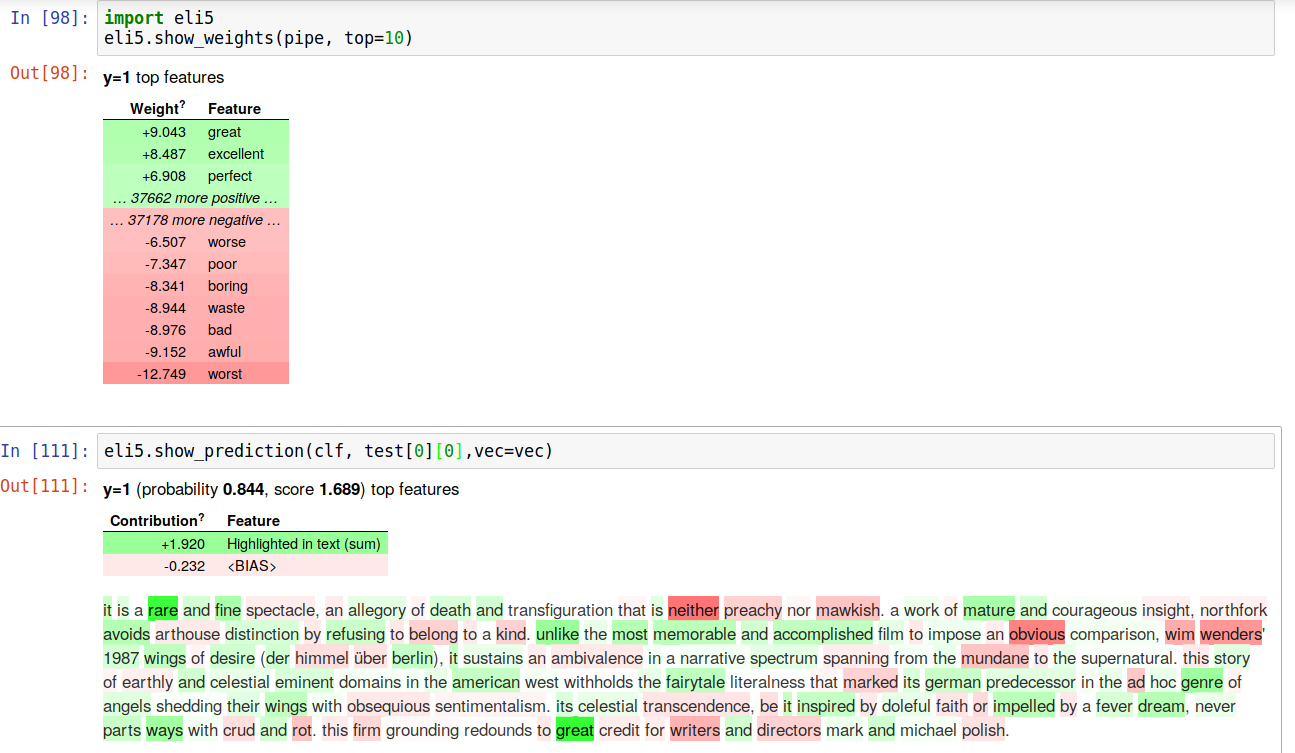
\includegraphics[width=\paperwidth,height=\paperheight,keepaspectratio]{../pictures/eli5}}
(example using the classifier \texttt{clf}, vectorizer \texttt{vec}, and pipeline \texttt{pipe} from privious slides)
\end{frame}



\subsection{Last suggestions}

\begin{frame}[plain]
\textbf{From feature set to final classification}

Last suggestions
\end{frame}


\begin{frame}{Some further ideas to look into}

\begin{block}{Balancing classes}
Your classifier probably works better if you have approximately the same amount of annotated training data for both classes (e.g., pos/neg). If getting such data is not an option, you may consider weighing accordingly, e.g. using

\texttt{LogisticRegression(class\_weight='balanced')}
\end{block}

\end{frame}

\begin{frame}{Some further ideas to look into}

\begin{block}{More advanced pipelines}
Consider constructing advanced pipelines, including a dimension reduction step: 


\url{https://scikit-learn.org/stable/tutorial/statistical\_inference/putting\_together.html}
\end{block}

\end{frame}



\begin{frame}{Some further ideas to look into}

\begin{block}{Combine different feature sets}
E.g, use BOW-features as well as features such as sentence length, number of sentences (or whatever)


\url{
https://scikit-learn.org/stable/auto\_examples/hetero\_feature\_union.html}
\end{block}

\end{frame}


\section{Advanced ML}


\begin{frame}[plain]
\vspace{2cm}
\textbf{Advanced Machine Learning techniques} \\
Embeddings and Keras
\vspace{2cm}
\end{frame}


\subsection{Embedding-based vectorizer}

\begin{frame}{Embedding based vectorizer}

\begin{block}{General idea}
	\begin{itemize}[<+->]
		\item language models that capture the meaning of words
		\item Similar words occupy similar positions
		\item Embedding models represent words in a high dimensional space 
	\end{itemize}
\end{block}

\pause
\begin{exampleblock}{Value for ML}
	\begin{itemize}
		\item Embedding models can help understand words in the application text even if they do \textcolor{red}{NOT} appear in the training data set
	\end{itemize}
\end{exampleblock}
\end{frame}


\begin{frame}[plain]
\textbf{Vectorizing data using embedding models}
\end{frame}

\begin{frame}{Embedding vectorizers}
\begin{block}{Embedding-based vectorizers}
	\begin{itemize}[<+->]
		\item For each word in a document, the associated word vectors in the embedding model are retrieved. 
		\item These features can weighted: 
		\begin{enumerate}
			\item average word frequency: \textcolor{red}{count}
			\item \textcolor{red}{tfidf} weighting
	\end{enumerate}
	\end{itemize}
\end{block}
\end{frame}

\begin{frame}[fragile]{Vectorize data using embedding model}
\begin{lstlisting}
import embeddingvectorizer
import gensim

model = gensim.models.Word2Vec.load(`path_to_w2v_model')  
embedding_mdl = dict(zip(model.wv.index2word, model.wv.syn0)) 
embedding_vect = embeddingvectorizer.EmbeddingCountVectorizer(embedding_mdl, `mean') 

\end{lstlisting}

{\footnotesize 
	\begin{description}
		\item[\textcolor{red}{embeddingvectorizer}] pip install embeddingvectorizer: \url{github.com/ccs-amsterdam/embeddingvectorizer} 
	\end{description}
}

\end{frame}

\begin{frame}[fragile]{Next step: Fit the model}
\begin{lstlisting}

from sklearn.linear_model import LogisticRegressionCV
from sklearn.pipeline import make_pipeline

clf = LogisticRegressionCV()
pipe = make_pipeline(embedding_vect, clf)
pipe.fit(X_train, y_train)
pipe.score(X_test, y_test)
\end{lstlisting}

\end{frame}

\begin{frame}[plain]
\huge

TODO
meer visualization
keras


\end{frame}








\end{document}
